% vim: spell spl=pt fo+=cwq tw=78 nonu sw=4 ts=4
% vim: fen fdc=1 fdm=marker fmr={{{,}}}

% sbc {{{
\documentclass[12pt]{article}
% }}}
% abnt {{{
%\documentclass{abnt}
% }}}
% packages {{{
\usepackage[portuguese,brazil,brazilian]{babel}
\usepackage[utf8]{inputenc}
\usepackage[T1]{fontenc}
\usepackage{graphicx}
\usepackage{epstopdf}
%\usepackage{wrapfig}
%\usepackage{caption}
\usepackage{float}
\usepackage{url}
%\usepackage[hypcap]{caption}
\usepackage{algorithm}
\usepackage{algpseudocode}
\usepackage{mathtools}
\usepackage{amsmath}
% }}}
% sbc {{{
\usepackage{sbc-template}
%}}}
% abnt {{{
%\usepackage[num]{abntcite}
% }}}
\usepackage[bookmarks]{hyperref}
%\usepackage[chapter]{algorithm}
     
\sloppy


% sbc {{{
\title{Handover Entre Redes Heterogêneas: Um Estudo de Casos do Padrão 
802.21}
\author{Higor Eurípedes P. F. A.\inst{1}, Cláudio de C. Monteiro\inst{1}}
\address{Instituto Federal de Educação, Ciência e Tecnologia do Tocantins 
	(IFTO)\\
  77.021-090 -- Palmas -- TO -- Brazil
  \email{heuripedes@gmail.com, ccm@ifto.edu.br}
}
\date{Junho, 2012}
% }}}
% abnt {{{
%\titulo{Transições Interrede Independentes do Meio Físico de Acesso}
%\autor{Higor Eurípedes P. F. A.}
%\orientador{Cláudio de C. Monteiro}
%\instituicao{Instituto Federal de Educação, Ciência e Tecnologia do Tocantins}
%\local{Palmas -- TO -- Brasil}
%\data{Fevereiro, 2012}
% }}}

\begin{document}


\floatname{algorithm}{Algoritmo}
\renewcommand{\algorithmicfunction}{\textbf{função}}
\renewcommand{\algorithmicprocedure}{\textbf{procedimento}}
\renewcommand{\algorithmicrequire}{\textbf{Require:}}
\renewcommand{\algorithmicensure}{\textbf{Ensure:}}
\renewcommand{\algorithmicend}{\textbf{fim}}
\renewcommand{\algorithmicif}{\textbf{se}}
\renewcommand{\algorithmicthen}{\textbf{então}}
\renewcommand{\algorithmicelse}{\textbf{senão}}
%\renewcommand{\algorithmicelsif}{\algorithmicif\ \algorithmicelse}
%\renewcommand{\algorithmicendif}{\algorithmicend\ do \algorithmicif}
\renewcommand{\algorithmicfor}{\textbf{para}}
\renewcommand{\algorithmicforall}{\textbf{para todo}}
\renewcommand{\algorithmicdo}{\textbf{faça}}
%\renewcommand{\algorithmicendfor}{\algorithmicend\ do \algorithmicfor}
\renewcommand{\algorithmicwhile}{\textbf{enquanto}}
%\renewcommand{\algorithmicendwhile}{\algorithmicend\ do \algorithmicwhile}
\renewcommand{\algorithmicloop}{\textbf{loop}}
%\renewcommand{\algorithmicendloop}{\algorithmicend\ \algorithmicloop}
\renewcommand{\algorithmicrepeat}{\textbf{repita}}
\renewcommand{\algorithmicuntil}{\textbf{até que}}
%\renewcommand{\algorithmicprint}{\textbf{imprima}}
\renewcommand{\algorithmicreturn}{\textbf{retorne}}
%\renewcommand{\algorithmictrue}{\textbf{verdade}}
%\renewcommand{\algorithmicfalse}{\textbf{falso}}



% sbc {{{
\maketitle
% }}}
% abnt {{{
%\capa
%\folhaderosto
%\sumario
% }}}

\begin{resumo}

O surgimento dos dispositivos multi interface, tornou possível o acesso 
ininterrupto a serviços, porém a estrutura lógica em uso se mostrou 
despreparada para esta nova demanda.

Este artigo, apresenta o padrão IEEE 802.21 de transições independentes do 
meio e propõe uma implementação distribuída baseada num subconjunto dos 
conceitos do mesmo.

\end{resumo}

\begin{abstract}

The emerging multi-interface device market, has made possible the seamless 
access to services based on general purpose networks, but the logic structure 
of the in-use techniques has proved unprepared to this new demand.

This paper, introduces the IEEE 802.21 standard for media independent handover 
and proposes a distributed implementation based on a subset of the concepts 
presented on the said standard.

\end{abstract}

% abnt {{{
%\chapter{Introdução}
% }}}

\section{Introdução} \label{sec:introducao} % {{{

A crescente procura por mobilidade impulsionou a venda de dispositivos móveis.  
Cada vez mais exigentes, os usuários demandam do mercado dispositivos que os 
permitam proceder com suas atividades onde e como lhe convir. Estas pessoas, 
em geral, gastam boa parte de seu dia utilizando ferramentas dependentes da 
\textit{Internet} e, portanto, precisam de soluções que lhes permitam dispôr 
da portabilidade de seus dispositivos ao realizar estas atividades.

Para atender esta demanda, tecnologias de comunicação sem fio como 
\textit{WiFi}, \textit{WiMAX} e 3g (\textit{3GPP} e \textit{3GPP2}) foram 
desenvolvidas.  Entretanto, com o surgimento de dispositivos capazes de se 
conectar com mais de uma rede ou tecnologia, a infraestrutura se mostrou 
deficiente quanto à integração destas tecnologias. Um dos motivos para que 
isto acontecesse, segundo \cite{piri:2009}, era a falta de padronização dos 
mecanismos de \textit{handover}.  

Como solução para esta situação, foi proposto o padrão IEEE 802.21  
\cite{ieee:2008:80221}, intitulado \textit{Media Independent Handover 
Services}. Este padrão, documenta mecanismos auxiliares para transição entre 
redes heterogêneas e seu objetivo principal é facilitar o processo de 
\textit{handover}, por meio de uma abstração das camadas inferiores chamada 
\textit{Media Independent Handover Function} (MIHF).

Nas seções seguintes, serão apresentados uma visão geral do padrão 802.21, de 
alguns trabalhos relacionados e, por fim, uma proposta de implementação de 
mecanismos do padrão IEEE 802.21.

%Nas quatro seções seguintes, estão presentes a justificativa, a problemática, 
%os objetivos e a metodologia utilizada nesta pesquisa, respectivamente. A 
%seção seção 6 apresenta uma visão geral do padrão, e em seguida são 
%apresentados os detalhes de uma proposta de implementação do mesmo.
%}}}

\section{Visão geral do padrão IEEE 802.21} \label{sec:padrao}  % {{{

O padrão tem o objetivo de assistir o processo de \textit{handover}. O 
elemento principal do padrão, segundo \cite{piri:2009}, é a entidade lógica 
MIHF, que se localiza entre as camadas de enlace e de rede e que abstrai a 
funcionalidade e as características da camada de enlace.  Esta entidade, é 
composta do serviço de controle, \textit{Media Independent Command Service} 
(MICS); do serviço de notificação de eventos, \textit{Media Independent Event 
Service} (MIES); e do serviço de informação, \textit{Media Independent 
Information Service} (MIIS):

\begin{itemize}

	\item O MICS, é, principalmente, responsável pela configuração de enlaces 
		e da realização dos \textit{handovers}, contudo, este serviço também é 
		utilizado para obtenção de informações dinâmicas como qualidade do 
		sinal e velocidade do enlace.

	\item O MIES, é responsável pela propagação e notificação de eventos de enlace 
		e de \textit{handover}. Estes eventos, são utilizados como gatilhos para 
		os \textit{handovers}.

	\item O MIIS, funciona como um repositório de informações sobre o móvel e 
		sobre o ambiente.  Estas informações, são utilizadas para guiar os 
		dispositivos durante o processo de \textit{handover}. O serviço pode 
		conter desde informações sobre o enlace até posicionamento do dispositivo 
		no ambiente.
	
\end{itemize}

De acordo com \cite{ieee:2008:80221}, a comunicação entre MIHFs e o 
\textit{usuário MIH} é feita utilizando-se um protocolo baseado em troca de 
mensagens chamado \textit{Media Independent Handover Protocol} (MIHP).  A 
comunicação, em geral, é feita de forma assíncrono (requisição e resposta). 
Porém o protocolo também suporta comunicação síncrona e o método 
\textit{push}, onde uma MIHF envia uma mensagem mesmo sem solicitação.  Os 
dados nos pacotes do MIHP (\textit{payload}), podem vir codificados em  TLV  
\footnote{\textit{type-length-value}, um formato binário em que cada 
informação possui identificador de tipo, tamanho e valor.} ou RDF 
\footnote{\textit{resource-description-framework}, um formato baseado em XML 
para a descrição de recursos.}.
% }}}

\section{Trabalhos relacionados} \label{sec:trabalhos} %{{{

O trabalho de \cite{tawil:2008}, propõe e analisa o comportamento de um 
processo distribuído de \textit{handover} vertical (DVHDS). Na avaliação, uma 
estação móvel se movimenta num ambiente simulado coberto por uma rede UMTS e 
quatro redes IEEE 802.11. Estas redes possuem suporte à serviços MIH e se 
encontram sobrepostas.

\begin{figure}[h!]
	\begin{minipage}[b]{0.5\linewidth}
		\centering
		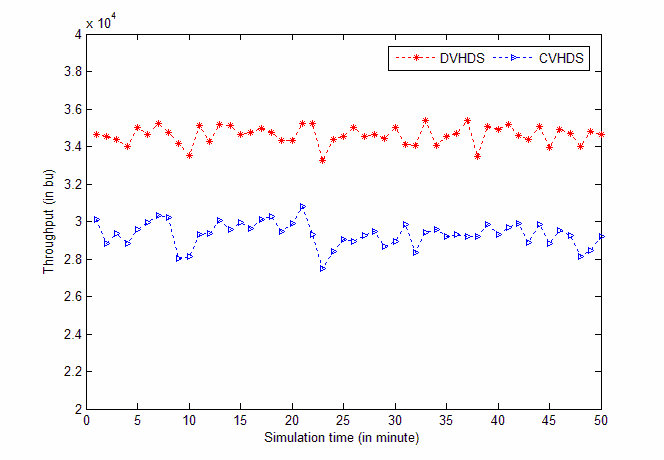
\includegraphics[width=\textwidth]{artigo-junho/dvhds-throughput.png}
		\caption{Rendimento de rede ao longo do tempo.}
		\label{fig:dvhds-throughput}
	\end{minipage}
	\begin{minipage}[b]{0.5\linewidth}
		\centering
		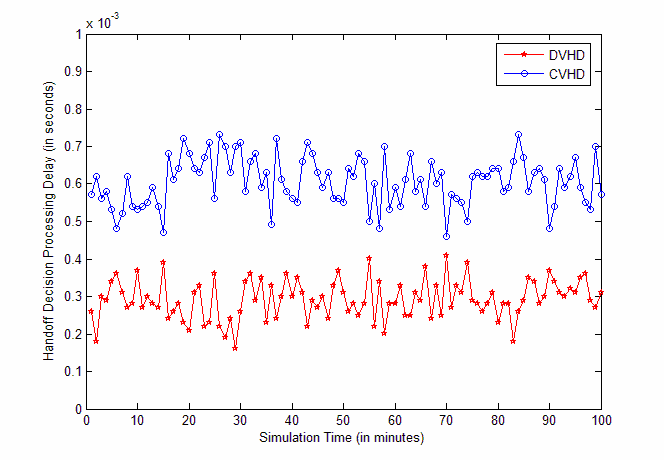
\includegraphics[width=\textwidth]{artigo-junho/dvhds-procdelay.png}
		\caption{Tempo de processamento ao longo do tempo.}
		\label{fig:dvhds-procdelay}
	\end{minipage}
\end{figure}

O esquema de \cite{tawil:2008}, se caracteriza como distribuído, porque boa 
parte da tomada de decisão é constituída pelo cálculo de \textit{índices de 
qualidade} (NQV) por parte das estações servidoras de possíveis redes alvo. A 
obra destaca a eficiência deste processo em relação aos processos 
centralizados, em termos de rendimento de rede e tempo de tomada de decisões, 
como apresentado nas figuras \ref{fig:dvhds-throughput} e 
\ref{fig:dvhds-procdelay}.  

Os índices de qualidade de rede, levam em conta os atributos da rede (largura 
de banda e custo monetário, por exemplo), e a importância, ou peso, que o 
usuário dá a cada um desses atributos. Após o cálculo, a rede de maior NQV se 
torna a rede alvo do \textit{handover}. O NQV pode ser calculado a partir da 
fórmula

\begin{align*}
	NQV_i &= \sum_{i=1,j=1}^{N,n_p^+}W_j * P_{ij} + \sum_{i=1,k=1}^{N,n_{p'}^-}W_k * \frac{1}{P'_{ik}}\\
	\text{onde}~NQV_i &= \text{indice de qualidade da $i$-ésima rede}, \\
	P_{ij} &= \text{fator benéfico}, \\
	P'_{ik} &= \text{fator maléfico}, \\
	W_j \text{e}~W_k &= \text{pesos de $P_{ij}$ e $P'_{ik}$}, \\
	N &= \text{número de redes}, \\
	n_p^+ \text{e}~n_p^- &= \text{número de fatores benéficos e maléficos.}
\end{align*}

%\begin{figure}[h!]
%	\centering
%	\includegraphics[width=.7\textwidth]{artigo-junho/machan.eps}
%	\caption{Tempo de handover em relação à carga de rede.  
%	(\cite{machan:2008})}
%	\label{fig:machan}
%\end{figure}

A obra de \cite{machan:2008}, é caracterizada por um ambiente urbano simulado, 
onde estações móveis se movimentam entre uma rede IEEE 802.11 e uma rede UMTS.  
O esquema também utiliza a tecnologia Mobile IPv6 (MIPv6), para endereçamento 
independente do ponto onde o móvel está conectado. O foco da obra é a 
avaliação do \textit{handover} do padrão IEEE 802.21, em especial o 
\textit{soft-handover}.

Os resultados da avaliação de \cite{machan:2008}, mostram a importância do 
suporte ao \textit{soft-handover} do padrão IEEE 802.21, caracterizado pela 
propagação do evento \textit{MIH Link Going Down} quando o enlace se degrada.
Em suas medições, \cite{machan:2008} notou que os \textit{handovers} eram, em 
média, 8\% mais rápidos quando o \textit{soft-handover} era utilizado. Além 
disso, nas situações onde ocorreu \textit{hard-handover}, houve um aumento 
médio de 5\% no tráfego das redes envolvidas.


% }}}

\section{Proposta} \label{sec:proposta} % {{{

A pesquisa se propõe a implementar um esquema distribuído de \textit{handover} 
inspirado nas ideias apresentadas, principalmente, nos trabalhos de  
\cite{machan:2008} e \cite{tawil:2008}. Pretende-se avaliar a proposta num 
ambiente real.

O ambiente, onde a proposta será testada, é composto por duas redes que se 
sobrepõem, uma utiliza a tecnologia IEEE 802.11 e a outra a tecnologia celular 
3G.  Neste ambiente, estão presentes uma estação móvel, uma \textit{Base 
Station} (BS) 802.11 \textit{handover} e uma BS 3G.  No esquema, a BS 802.11 e 
a estação móvel possuem interfaces 3G e suporte a MIH, já a BS 3G, não terá 
suporte a MIH, pois esta faz parte de uma rede proprietária e não possuímos 
acesso interno à mesma.

\begin{figure}[h!]
	\centering
	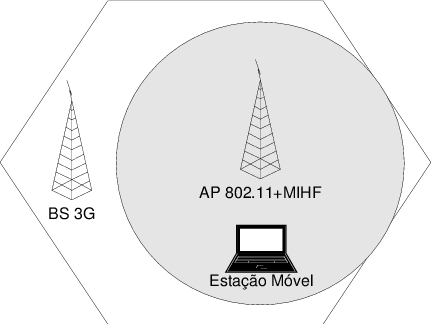
\includegraphics[width=.5\textwidth]{artigo-junho/ambiente.eps}
	\caption{Ambiente proposto.}
	\label{fig:ambiente}
\end{figure}

Optou-se por organizar o ambiente deste modo, por permitir a demonstração do 
mecanismo de \textit{soft-handover} do padrão 802.21 
(\textit{MIH\_Link\_Going\_Down}), quando o móvel se distancia da BS 802.11; e 
da escolha de redes mais rápidas ou confiáveis, quando o móvel entra na área 
de cobertura da BS 802.11.

\subsection{A MIHF e as primitivas MIH} %{{{

A MIHF proposta terá dois modos de operação, servidor e cliente.  A diferença 
principal entre os dois modos de operação, reside na forma como são tratadas 
certas primitivas.  Nesta MIHF, estarão presentes os três serviços MIH 
descritos em \cite{ieee:2008:80221}, porém com número de primitivas reduzido 
(tabela \ref{tab:primitivas}). A redução permite que a implementação 
restrinja-se somente aos itens mais relevantes do processo de 
\textit{handover}: a notificação do evento de quebra ou degradação do link e o 
comando para a troca de link. Abaixo está a descrição das primitivas 
introduzidas na implementação:

\begin{table}[ht]
	\centering
	\caption{Primitivas do esquema proposto}
	\label{tab:primitivas}
	\begin{tabular}[ht]{ l | l | l }
		Primitiva & Serviço & Descrição \\
		\hline
		MIH\_Link\_Up          & MIES & O enlace foi estabelecido.  \\
		MIH\_Link\_Down        & MIES & O enlace foi quebrado.  \\
		MIH\_Link\_Going\_Down & MIES & O enlace se degradou. \\
		MIH\_Link\_Switch      & MICS & Realiza o \textit{handover}. \\
		MIH\_Report          & MIIS & Consulta informações sobre enlaces. \\
		MIH\_Discovery   & MICS & Procura MIHFs servidoras na rede.  \\
		\hline
	\end{tabular}
	
\end{table}

\begin{enumerate}

	\item MIH\_Link\_Switch -- Esta primitiva é utilizada para realizar a 
		transição entre links. Substitui a funcionalidade das primitivas 
		MIH\_Net\_HO\_*, MIH\_N2N\_HO\_*, MIH\_MN\_HO\_* e 
		MIH\_Link\_Handover\_*.
	
	\item MIH\_Report -- Esta primitiva é utilizada para solicitar informações 
		sobre redes disponíveis às estações servidoras. Substitui a 
		funcionalidade das primitivas MIH\_Get\_Information, 
		MIH\_Link\_Get\_Parameters e MIH\_Link\_Parameters\_Report.
	
	\item MIH\_Discovery -- Esta primitiva é utilizada para descobrir
		pontos de acesso numa determinada rede. Uma requisição é enviada por 
		\textit{broadcast} ou \textit{multicast} e estações servidoras deverão 
		responder informando os links disponíveis. Estações cliente deverão 
		ignorar estas requisições. Substitui a funcionalidade da primitiva
		MIH\_Register.

\end{enumerate}

A subscrição de eventos e o registro de \textit{peers} é feita automaticamente 
pela MIHF servidora, assim que recebe uma requisição MIH\_Discovery. O 
\textit{MIH User} também está dispensado da tarefa de subscrição, visto que a 
MIHF estará integrada e por definição todo evento de link recebido será 
repassado a ele.

Enquanto eventos como \textit{MIH\_Link\_Down} e \textit{MIH\_Link\_Up} são 
gerados de forma intuitiva (ou o enlace está pronto para uso ou não está), o 
evento \textit{MIH\_Link\_Going\_Down} somente é disparado quando certo 
parâmetro ultrapassa o limiar configurado pelo \textit{MIH User} 
(\cite{ieee:2008:80221}). Este limiar, no presente esquema, estará 
pré-configurado na MIHF, visto que a mesma não terá suporte ao comando 
\textit{MIH\_Link\_Configure\_Thresholds}. Quanto ao evento 
\textit{MIH\_Link\_Going\_Down}, este será gerado sempre que a média da 
intensidade do sinal das ultimas dez medições for inferior ao limiar do 
enlace.

%}}}

\subsection{\textit{Handover}} %{{{

A notificação de sinais de enlace, dá oportunidades para que a implementação 
possa escolher a rede mais benéfica ao usuário. No esquema proposto, assume-se 
que a rede mais benéfica é aquela com sinal mais intenso ou de tecnologia mais 
confiável, assim como descrito no algoritmo \ref{algo:sel-rede}.

\begin{algorithm}
	\caption{Seleção de rede\label{algo:sel-rede}}
	\begin{algorithmic}[1]
		\Function{MelhorRede}{$R$, $a$}
			\State $M \gets$ Enlaces móveis presentes em R.
			\State $W \gets$ Enlaces WiFi presentes em R.
			\State $F \gets$ Intensidades dos sinais dos enlaces presentes em R.

			\ForAll{$r \in R$}

				\State $ar \gets \{a, r\}$

				\If{$((a \in M)$ \textbf{and} $(r \notin M))$ \textbf{or} 
				$((ar \subset M$ \textbf{or} $ar \subset W)$ \textbf{and} $F_r > F_a$)}

					\State $a \gets r$
					
				\EndIf

			\EndFor

			\State \Return{$a$}

		\EndFunction
	\end{algorithmic}
\end{algorithm}

\begin{figure}[ht]
	\centering
	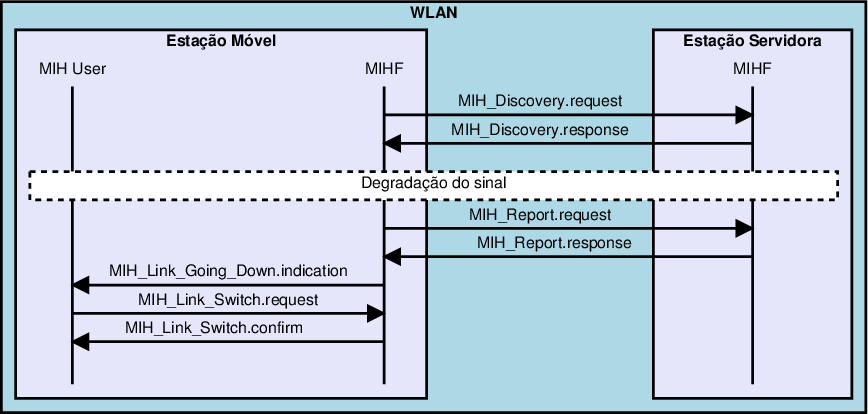
\includegraphics[width=0.8\textwidth]{artigo-junho/novo-soft-handover.eps}
	\caption{Processo de \textit{soft-handover}.}
	\label{fig:soft-handover}
\end{figure}

No processo de \textit{soft-handover}, um nó equipado com uma MIHF em modo 
servidor fornece ao cliente informações sobre as redes do ambiente (figura 
\ref{fig:soft-handover}.) Quando identifica a degradação do sinal, a MIHF 
cliente requisita à estação servidora uma lista de redes disponíveis por meio 
de MIH\_Report, ao receber a resposta, o cliente é notificado da degradação e 
recebe a lista retornada pela estação servidora. O cliente, então, seleciona a 
melhor conexão e solicita à sua MIHF que seja realizado o \textit{handover}.

%}}}

% }}}

\section{Materiais e Métodos} %{{{

\subsection{Material}

Para a implementação e avaliação da proposta, será utilizada a linguagem 
Python versão 2.7 e a distribuição Ubuntu. Serão utilizados na avaliação 
netbooks equipados com uma interface 3G (\textit{modem} USB) e WiFi (onboard).

\subsection{Método}

O desenvolvimento da proposta será feito utilizando prototipação, para 
permitir avaliações prévias sobre o estado do projeto em relação ao que foi 
planejado e para que sejam feitas correções (se necessárias) em tempo hábil.

Na maior parte do código, será utilizado o paradigma procedural, porém, em 
áreas que manipulam ou dependem muito de estado, será utilizado o paradigma de 
programação orientada a objetos. A escolha de uma implementação 
multi-paradigma foi feita por proporcionar facilidade na codificação sem 
comprometimento da complexidade.

A proposta será avaliada quanto ao tempo de \textit{handover} em determinadas 
condições, e pretende-se oferecer uma garantia de que, em 95\% dos casos, a
duração das transições sejam feitas no tempo estimado pela a avaliação. Para 
atingir esse nível de confiança, será preciso coletar dados sobre uma amostra 
preliminar de \textit{handovers}, os quais serão utilizados no cálculo da 
amostra populacional necessária para atingir 95\% de confiança.


\section{Resultados e Discussão}

Os algoritmos da proposta, são, de um modo geral, inocentes e podem apresentar 
problemas em casos extremos. O algoritmo de seleção de rede 
\ref{algo:sel-rede}, por exemplo, não leva em consideração parâmetros como a 
latência e a segurança na hora de escolher a melhor rede.

A forma como as informações locais são captadas e manipuladas pelas MIHFs da 
proposta, também podem causar problemas. Se for utilizado um método de 
\textit{polling} inadequado, os algoritmos \ref{algo:monitor} e \ref{algo:lgd} 
podem apresentar problemas de concorrência que deixariam o móvel sem conexão 
durante um \textit{handover}.

\noindent\begin{minipage}[h]{\textwidth}
	\resizebox{.5\textwidth}{!}{%
	\begin{minipage}[t]{.75\textwidth}
		\begin{algorithm}[H]
			\caption{Monitoramento de links \label{algo:monitor}}
			\begin{algorithmic}[1]
				\Procedure{Monitorar}{}
				
				\State $L \gets$ Links monitorados.
				\State $L' \gets$ Links locais disponíveis.
				\State $N \gets L' \setminus L$ \Comment{Links novos}
				\State $M \gets L \setminus L'$ \Comment{Links "mortos"}

				\State $L \gets (L \setminus M) \cup N$	

				\ForAll{$l \in M$}% \Comment{Notifica o usuário MIH sobre links mortos}
					\State $MihLinkDown(l)$
				\EndFor

				\ForAll{$l \in N$}% \Comment{Notifica o usuário MIH sobre links novos}
					\State $MihLinkUp(l)$ 
				\EndFor
				
				%\ForAll{$l \in L$} \Comment{Atualiza informações sobre os links}
				%	\State $AtualizarLink(l)$
				%\EndFor
				\EndProcedure
				
			\end{algorithmic}
		\end{algorithm}
	\end{minipage}
	}
	\resizebox{.5\textwidth}{!}}}

\section{Conclusão} %{{{

O esquema proposto, por possuir um escopo reduzido, se mostra viável em termos 
acadêmicos.  Porém, há de se notar que o mesmo possui algumas deficiências, 
como, por exemplo, a necessidade de o móvel deixar suas interfaces ligadas 
quando fora do alcance da rede com suporte a MIH.

Apesar de se mostrar propício à implementação, o esquema proposto teria 
dificuldades de se adequar ao mundo real, isto é, fora do propósito ao qual 
foi concebido. O motivo principal é que o mesmo, em prol da simplicidade, se 
desvia do estabelecido no padrão IEEE 802.21 e por isso se torna incompatível 
com implementações que o sigam à risca.

A existência da MIHF servidora, e dos esquemas distribuídos de 
\textit{handover} em geral, é uma faca de dois gumes.  As informações 
levantadas pela MIHF servidora podem não se encaixar na condição do móvel ou 
levá-lo a tomar decisões incorretas, visto que estas informações tem origem em 
um ponto de de vista diferente do ambiente. Entretanto, quando implementada em 
ambientes propícios, a MIHF servidora oferece um grande beneficio à computação 
móvel, vide resultados de \cite{tawil:2008} e a possibilidade de o móvel 
economizar bateria quando sob a cobertura da rede com suporte a MIH do esquema 
proposto.

%Este artigo propôs um esquema distribuído de \textit{handover}, utilizando 
%conceitos presentes no padrão IEEE 802.21. Como pôde ser visto, o esquema 
%proporciona ao móvel economia de recursos ao repassar parte da 
%responsabilidade do \textit{handover} à estação servidora. Foram apresentados 
%também, os efeitos da utilização de esquemas distribuídos e do suporte a 
%\textit{soft-handover}.

%}}}

%
%\section{FIXME}
%
%\textbf{FIXME}: inconsistência(?): o móvel terá de ficar com as duas 
%interfaces ligadas quando estiver fora da rede 802.11?
%
%\textbf{FIXME}: inconsistência/contradição(?): como posso dizer que a proposta 
%serve para demonstrar funcionalidade do padrão se ela só implementa 0.01\% 
%dele, introduz coisas não documentadas e ainda é incompatível com o protocolo 
%documentado?



%}}}




% primitivas
%mies --
%mih link up (indication: <node, id>)
%mih link down (indication: <node, id>)
%mih link going down (indication: <node, id>)
%
%mics --
%mih ho_commit (comando: <oldnet, newnet> indication: <node, oldnet, newnet>)
%mih report (request: <node> response: <node, {link1: {id, mac, ip} ...})
%
%miis --
%mih net discovery (request: response: <node>)


\bibliographystyle{sbc}
%\bibliographystyle{abnt-num}

\bibliography{artigo-junho}


\end{document}
